\documentclass{beamer}
\usetheme{UWr_white}

\usepackage{polski}
\usepackage[utf8]{inputenc}
\usepackage{color,graphicx}
\usepackage{amssymb}
\usepackage{enumerate}
\usepackage{amsmath}
\usepackage{caption}
\usepackage{subcaption}
\usepackage{geometry}
\usepackage{empheq}
\usepackage{wrapfig}
\usepackage{float}
\usepackage{changepage}
\usepackage{hyperref}

\newcommand{\Leo}{\mathcal{L}_{\varepsilon}}

\theoremstyle{break}
	\newtheorem{thm}{Theorem}[section]
\theoremstyle{break}
	\newtheorem{asm}{Assumption}[section]
\theoremstyle{break}
	\newtheorem{rem}{Remark}[section]
\theoremstyle{break}
	\newtheorem{lem}{Lemma}[section]
\theoremstyle{break}
	\newtheorem{defi}{Definition}[section]
 
\title{Jak grzać?}
\author{Maciej Tadej}

\institute{\textit{Instytut Matematyczny, UWr, Poland \\ Center for Advanced Systems Understanding, HZDR, Germany}}

\setbeamercovered {invisible}

\begin{document}

\begin{frame}
	\titlepage{}
\end{frame}

\section{Wprowadzenie}

\begin{frame}{Olimpiada Sztucznej Inteligencji}
    \begin{figure}[ht]
        \centering
        
\includegraphics[width=\linewidth]{imgs_pres/Partnerzy Instytucjonalni.png}
        \label{fig:enter-label}
    \end{figure}
\end{frame}

\begin{frame}{O co chodzi?}
    \begin{itemize}
        \item W związku z dynamiczną sytuacją międzynarodową, \textbf{ceny energii rosną w zawrotnym tempie}
        \item Opcji na rozwiązanie tego problemu jest kilka, na przykład:
        \begin{itemize}
            \item nie grzać wcale
            \item oszczędzać (głupio)
            \item oszczędzać (mądrze)
        \end{itemize}
        \item Aby oszczędzać mądrze, trzeba posłużyć się pewnymi narzędziami \ldots
    \end{itemize}
    
\end{frame}

\begin{frame}{Plan spotkania}
    \begin{itemize}
        \item Troszkę o fizyce i kaloryferach \ldots
        \item Jak przełożyć to co powie fizyk na język matematyki?
        \item Wzorów nie ma, ale też jest fajnie.
    \end{itemize}
\end{frame}

\section{Ogrzewanie z perspektywy fizyki}


\begin{frame}{Czym jest ciepło?}
    
    \begin{itemize}
        \item \textbf{Ciepło to forma energii} przekazywana między ciałami na skutek różnicy temperatur.
        \item Jednostką ciepła w układzie SI jest \textbf{dżul (J)}.
        \item Gdy ciało otrzymuje energię cieplną, jego temperatura rośnie, a gdy traci energię cieplną, jego temperatura spada.
    \end{itemize}
\end{frame}

\begin{frame}
    \frametitle{Czym jest temperatura?}

    \begin{itemize}
        \item \textbf{Temperatura to miara średniej energii kinetycznej} cząsteczek w układzie.
        \item Jednostką temperatury w układzie SI jest \textbf{kelwin (K)}.
        \item Temperatura wskazuje, czy i w jakim kierunku nastąpi przepływ ciepła między dwoma ciałami.
    \end{itemize}
\end{frame}

\begin{frame}{Ogrzewanie -- Jak to się dzieje?}
    
    \begin{itemize}
        \item \textbf{Transfer ciepła to proces przekazywania energii cieplnej} z jednego ciała lub miejsca do innego na skutek różnicy temperatur.
        \item Wyróżniamy trzy podstawowe mechanizmy transferu ciepła:
        \begin{itemize}
            \item \textbf{Dyfuzja / Przewodnictwo} - przenoszenie ciepła wewnątrz ciała stałego lub między ciałami w kontakcie.
            \item \textbf{Konwekcja / Adwekcja} - przenoszenie ciepła w wyniku ruchu płynów (cieczy i gazów).
            \item \textbf{Promieniowanie} - przekazywanie energii cieplnej w postaci fal elektromagnetycznych, bez potrzeby istnienia ośrodka materialnego.
        \end{itemize}
    \end{itemize}
\end{frame}

\begin{frame}{Ogrzewanie -- Jak to się dzieje?}
    \begin{figure}
        \centering
        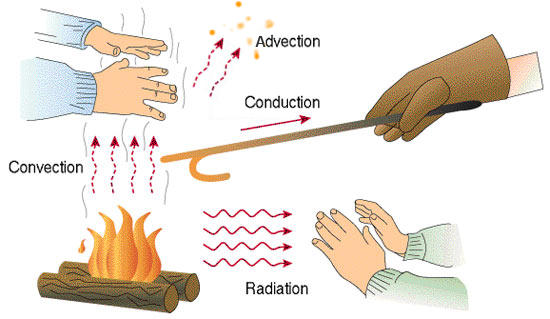
\includegraphics[width=0.7\textwidth]{imgs_pres/Heat-transmittance-means.jpg}
        \caption{
        \hyperlink{https://en.wikipedia.org/wiki/Advection#Distinction_between_advection_and_convection}{https://en.wikipedia.org/wiki/Advection\#Distinction-between-advection-and-convection}
        }
        \label{fig:enter-label}
    \end{figure}    
\end{frame}

\begin{frame}{Czym to się robi? - Kaloryfer CO/olejowy}
    \begin{figure}
        \centering
        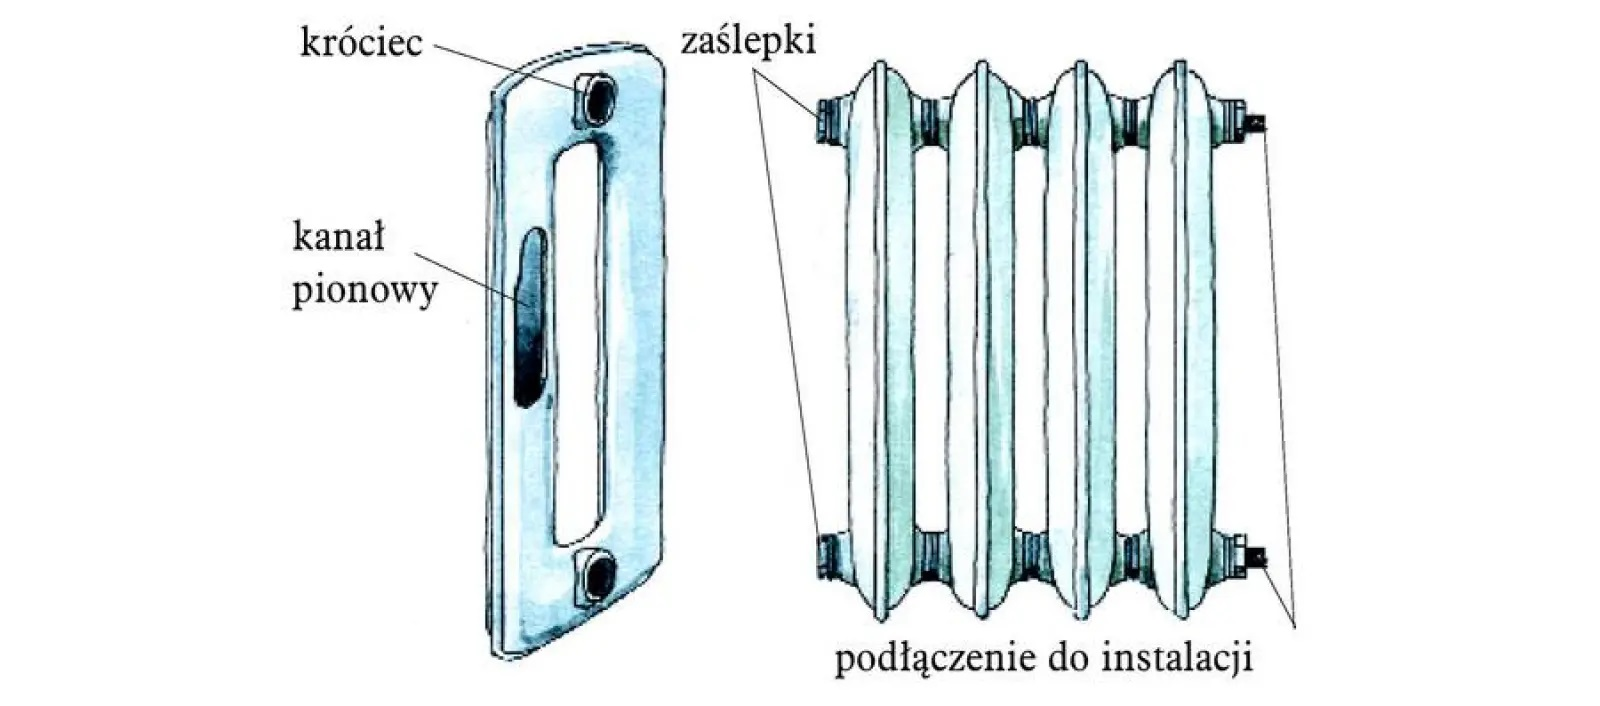
\includegraphics[width=\textwidth]{imgs_pres/schemat_grzejnik_żeliwny.jpg}
        \caption{\textit{https://budujemydom.pl/instalacje/ogrzewanie-podlogowe-i-grzejniki/a/512-nowoczesne-grzejniki-zeliwne}}
        \label{fig:enter-label}
    \end{figure}
\end{frame}

\begin{frame}{Czym to się robi? - Kaloryfer płytowy}
    \begin{figure}
        \centering
        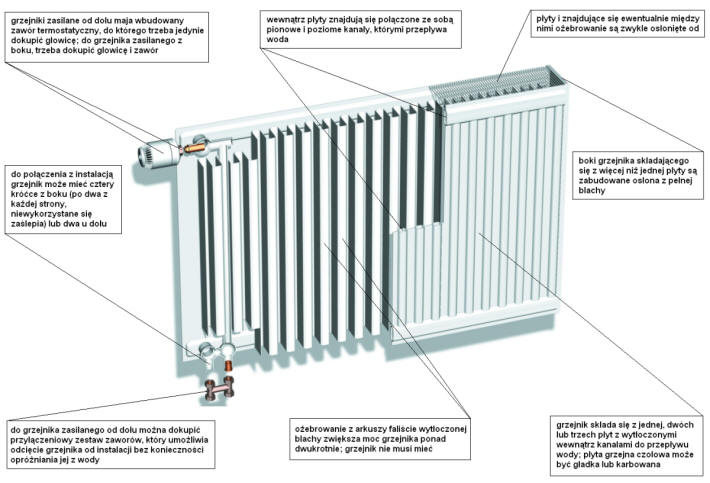
\includegraphics[width=0.7\textwidth]{imgs_pres/schemat_grzejnik_stalowy.jpg}
        \caption{https://instsani.pl/technik-inzynierii-sanitarnej/vademecum-instalacji-sanitarnych/instalacje-centralnego-ogrzewania/odbiorniki-ciepla-grzejniki/grzejniki-stalowe-plytowe/}
        \label{fig:enter-label}
    \end{figure}
\end{frame}

\begin{frame}{Ile ciepła potrzeba?}
    Do zmiany temperatury masy powietrza o \textbf{objętości} $V [m^3]$, \textbf{cieple właściwym} $c = 1005 \left[ \frac{J}{kgK} \right]$, \textbf{gęstości} $\rho = \rho(T)$ i \textbf{masie} $m \left[kg\right]$, o wartość $\Delta T \left[ K \right]$ należy wykonać pracę (dostarczyć, bądź oddać ciepło)
    \begin{equation*}
        Q = m \cdot c \cdot \Delta T = \rho \cdot V \cdot c \cdot \Delta T
    \end{equation*}
\end{frame}

\begin{frame}{Co to jest moc?}
    Bardzo ważnym pojęciem jest \textbf{moc} $P \left[ W \right]$ równa pracy wykonanej przed układ o objętości $V [m^3]$ w danym czasie $\Delta t \left[s\right]$. W tym wypadku
    \begin{equation*}
        P = \frac{Q}{\Delta t} = \rho \cdot V \cdot c \frac{\Delta T}{\Delta t}
    \end{equation*}
    Po przekształceniu:
    \begin{equation*}
        \frac{\Delta T}{\Delta t} = \frac{P}{\rho \cdot V \cdot c}
    \end{equation*}
\end{frame}

\begin{frame}{Matematyczny formalizm}
    \begin{itemize}
        \item Przyjmujemy, że $T := T(x, t)$ jest \textit{funkcją} temperatury określoną dla położenia w przestrzeni $x$ oraz czasu $t$
        \item Oznaczamy przez $\frac{\partial T}{\partial t}$ \textit{pierwszą pochodną} temperatury po czasie. Formalnie jest to granica przy zmianie w czasie $\Delta t$ dążącej do zera.
        \begin{equation*}
            \frac{\partial T}{\partial t}(x,t) = \lim_{\Delta t \rightarrow 0} \frac{\Delta T (x,t)}{\Delta t},
        \end{equation*}
        gdzie
        \begin{equation*}
            \Delta T(x,t) = T(x. t + \Delta t) - T(x, t), 
        \end{equation*}
        \item Analogicznie, przez $\frac{\partial T}{\partial x}$ \textit{pierwszą pochodną} temperatury po przestrzeni oraz przez $\frac{\partial^2 T}{\partial x^2}$ \textit{drugą pochodną} temperatury po przestrzeni
    \end{itemize}
\end{frame}

\begin{frame}{Fizyczna interpretacja}
    Pochodna mierzy jak bardzo zmienia się dana wielkość.
    \begin{itemize}
        \item $\frac{\partial T}{\partial t} \left[ \frac{K}{s} \right]$ - mierzy jak zmienia się temperatura w czasie
        
        \item $\frac{\partial T}{\partial x} \left[ \frac{K}{m} \right]$ - mierzy jak zmienia się temperatura w przestrzeni
        
        \item $\frac{\partial^2 T}{\partial x^2} \left[ \frac{K}{m^2} \right]$ - mierzy jak szybko zmienia się temperatura w przestrzeni
    \end{itemize}
\end{frame}

\begin{frame}{Model v0 -- Przewodnictwo Cieplne}
    \begin{equation*}
        \frac{\partial T}{\partial t} = \frac{P}{\rho_{powietrza} \cdot V_{kaloryfera} \cdot c_{powietrza}}
    \end{equation*}
\end{frame}

\begin{frame}{Model v1 -- Równanie Dyfuzji}
    \begin{equation*}
        \frac{\partial T}{\partial t} = \alpha \cdot \frac{\partial^2 T}{\partial x^2} + \frac{P}{\rho \cdot V \cdot c},
    \end{equation*}
    gdzie $\alpha \left[ \frac{m^2}{s} \right]$ to współczynnik dyfuzji cieplnej.
\end{frame}

% \begin{frame}{Fizyczny model v3}
%     \begin{equation*}
%         \frac{\partial T}{\partial t} = \alpha \cdot \frac{\partial^2 T}{\partial x^2} + \frac{P}{\rho_{powietrza} \cdot c} - \frac{\partial}{\partial x} (\textbf{v} \cdot T),
%     \end{equation*}
%     gdzie $\mathbf{v} \left[ \frac{m}{s} \right]$ to prędkość poruszającego się powietrza.
% \end{frame}

\begin{frame}{Model v2 -- A ściany i okna?}
    \begin{equation*}
        \frac{\partial T}{\partial t} = \alpha \cdot \frac{\partial^2 T}{\partial x^2} + \frac{P}{\rho \cdot V \cdot c},
    \end{equation*}
    Ponadto zakładamy, że
    \begin{itemize}
        \item Okna przyjmują temperaturę zewnętrzną,
        \item Ściany nie przepuszczają (za dużo) ciepła.
    \end{itemize}
\end{frame}

\section{Analiza numeryczna}

\begin{frame}{Rozważane scenariusze}
    \begin{itemize}
        \item Dlaczego grzejnik stoi pod oknem?
        \item Jak ogrzać zimny pokój?
        \item Po co grzać skoro sąsiad mnie grzeje?
    \end{itemize}
\end{frame}

\begin{frame}{Przykładowy schemat domu}
    \begin{figure}
        \centering
        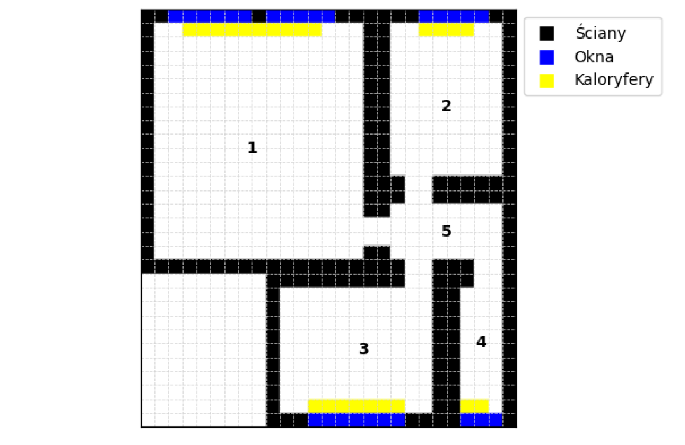
\includegraphics[width=\linewidth]{imgs_pres/house_scheme.jpg}
        \label{fig:enter-label}
    \end{figure}
\end{frame}

\begin{frame}{Jak to ugryźć komputerowo?}
    \begin{itemize}
        \item Modelowanie powierzchni za pomocą macierzy (siatek pomiarowych).
    \end{itemize}
    \begin{equation*}
        \begin{bmatrix}
        1 & 2 & 0 & 4 & 5 & 0 & 3 & 2 \\
        0 & 3 & 6 & 0 & 1 & 2 & 0 & 4 \\
        7 & 0 & 2 & 3 & 0 & 5 & 1 & 0 \\
        4 & 1 & 0 & 2 & 3 & 0 & 6 & 7 \\
        0 & 5 & 4 & 1 & 0 & 2 & 3 & 0 \\
        3 & 0 & 1 & 6 & 7 & 0 & 2 & 5 \\
        2 & 4 & 0 & 0 & 5 & 6 & 1 & 3 \\
        6 & 0 & 3 & 5 & 2 & 1 & 0 & 4 \\
        \end{bmatrix}
    \end{equation*}
\end{frame}

\begin{frame}{Liczenie pochodnych czasowych}
    \vfill
    Z definicji pochodnej mamy, że
    \begin{equation*}
        \frac{\partial T}{\partial t}(x,t) = \lim_{h_t \rightarrow 0} \frac{T(x, t + h_t) - T(x, t)}{h_t}
    \end{equation*}
    \begin{figure}[ht]
        \centering
        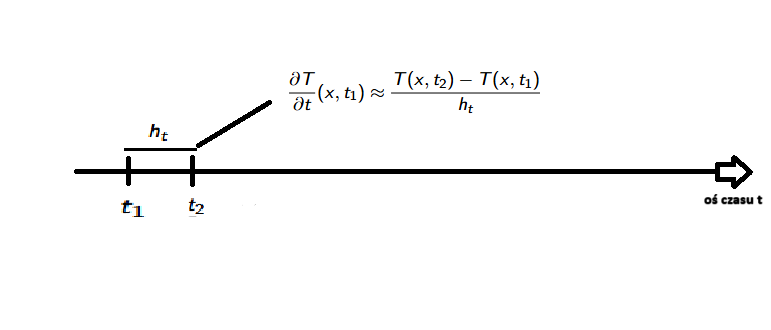
\includegraphics[width=0.9\linewidth, height=7.5cm]{imgs_pres/time_derivative.png}
        \label{fig:enter-label}
    \end{figure}
\end{frame}

\begin{frame}{Liczenie pochodnych przestrzennych}
    Z pewnych względów lepiej tutaj uwzględnić różnicę ze wszystkich stron
    \begin{align*}
        \frac{\partial T}{\partial x} 
        &= \lim_{h_x \rightarrow 0} \frac{1}{2} \left( \frac{T(x + h_x, t) - T(x, t)}{h_x} + \frac{T(x, t) - T(x - h_x, t)}{h_x}\right) \\
        &= \lim_{h_x \rightarrow 0} \frac{T(x + h_x, t) - T(x - h_x, t)}{2 \cdot h_x} \\
        \frac{\partial^2 T}{\partial x^2} 
        &= \lim_{h_x \rightarrow 0} \frac{\frac{\partial T}{\partial x}(x+h_x, t) - \frac{\partial T}{\partial x}(x-h_x, t)}{h_x} \\
        &\ldots \\
        &\approx \lim_{h_x \rightarrow 0} \frac{T(x-h_x, t) + T(x+h_x, t) - 2 T(x,t)}{h_x^2}
    \end{align*}
\end{frame}

\begin{frame}{Liczenie pochodnych przestrzennych}
    \begin{figure}[ht]
        \centering
        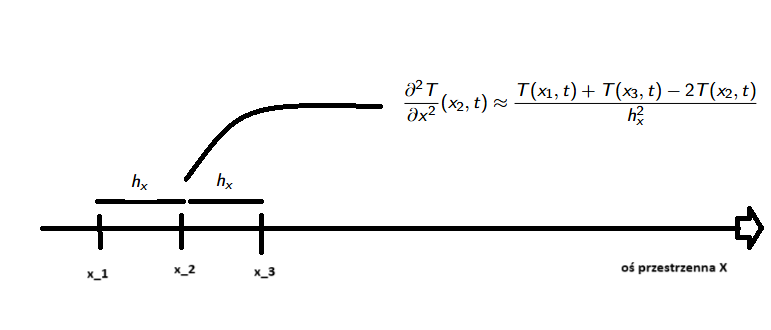
\includegraphics[width=\linewidth]{imgs_pres/space_derivative.png}
        \label{fig:enter-label}
    \end{figure}
\end{frame}

\section{Wnioski}

\begin{frame}{Rozważane scenariusze}
    \begin{itemize}
        \item \textbf{Dlaczego grzejnik stoi pod oknem?} - J. Chytła. \textit{Modelowanie deterministyczne 2024 / 2025}.
        \item Jak ogrzać zimny pokój?
    \end{itemize}
\end{frame}

\begin{frame}{Dlaczego grzejniki stoją pod oknem?}
    \begin{figure}[ht]
        \centering
        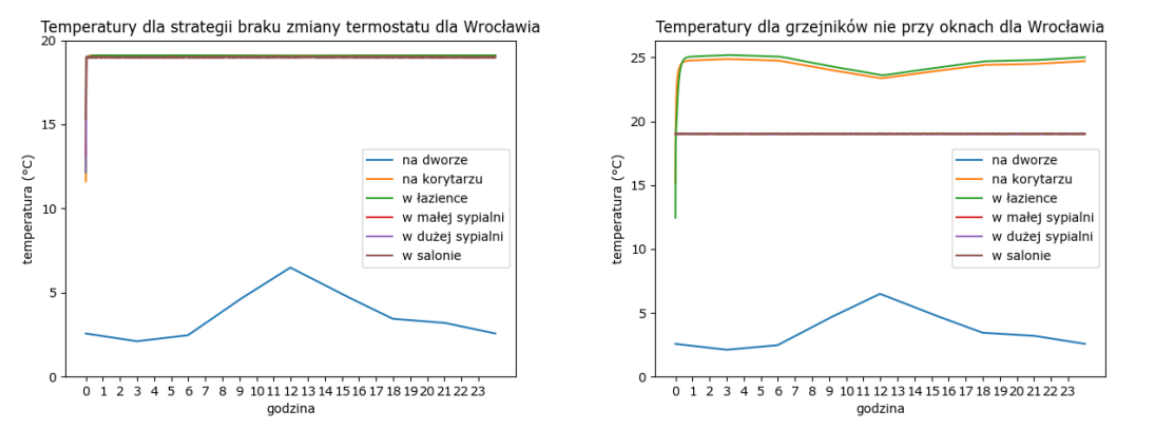
\includegraphics[width=\linewidth]{imgs_pres/gdzie_grzejnik_wroclaw.png}
        \label{fig:enter-label}
    \end{figure}
\end{frame}

\begin{frame}{Dlaczego grzejniki stoją pod oknem?}
    \begin{figure}[ht]
        \centering
        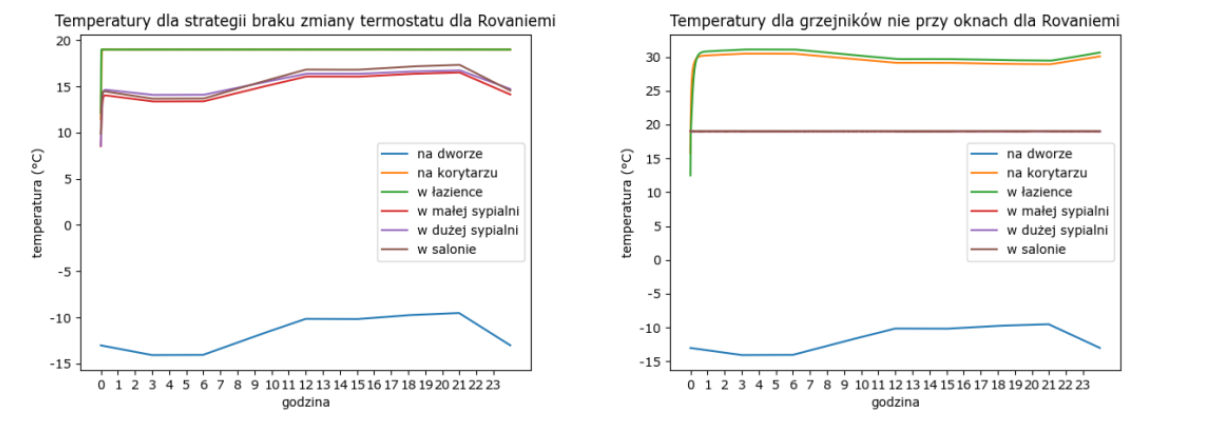
\includegraphics[width=\linewidth]{imgs_pres/gdzie_grzejnik_rovaniemi.png}
        \label{fig:enter-label}
    \end{figure}
\end{frame}

\begin{frame}{Wrocław, zużycie energii}
    \begin{figure}[ht]
        \centering
        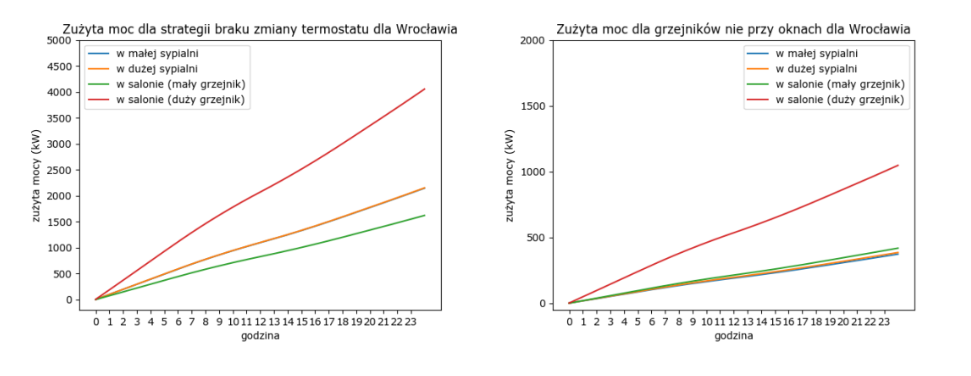
\includegraphics[width=\linewidth]{imgs_pres/grze_grzejnik_wroclaw_moz.png}
        \label{fig:enter-label}
    \end{figure}
\end{frame}

\begin{frame}{Rovaniemi, zużycie energii}
    \begin{figure}[ht]
        \centering
        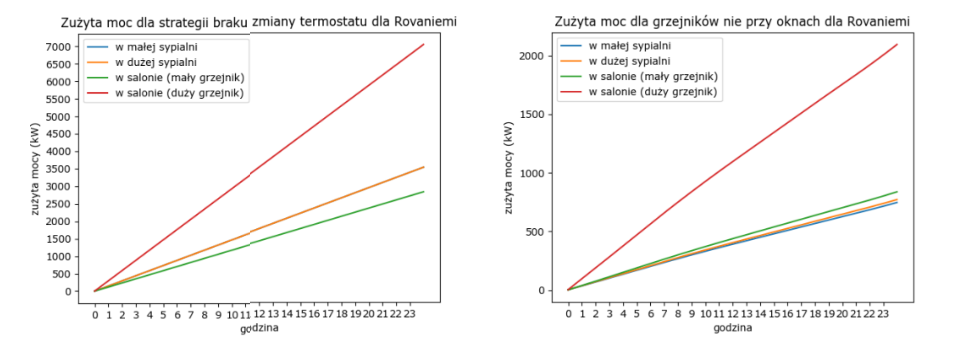
\includegraphics[width=\linewidth]{imgs_pres/grze_grzejnik_rowaniemi_moz.png}
        \label{fig:enter-label}
    \end{figure}
\end{frame}

\begin{frame}{Wrocław, temperatura o 0:30}
    \begin{figure}[ht]
        \centering
        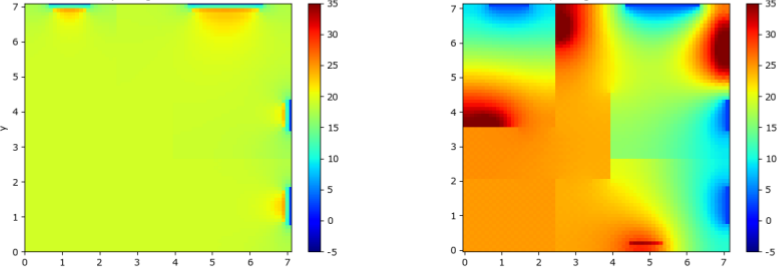
\includegraphics[width=\linewidth]{imgs_pres/wroclaw_temp_ostateczne.png}
        \label{fig:enter-label}
    \end{figure}
\end{frame}

\begin{frame}{Rovaniemi, temperatura o 0:30}
    \begin{figure}[ht]
        \centering
        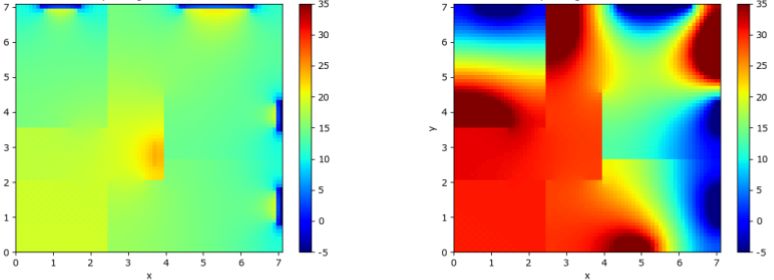
\includegraphics[width=\linewidth]{imgs_pres/rovaniemi_temp_ostateczne.png}
        \label{fig:enter-label}
    \end{figure}
\end{frame}

\begin{frame}{Rozważane scenariusze}
    \begin{itemize}
        \item Dlaczego grzejnik stoi pod oknem?
        \item \textbf{Jak ogrzać zimny pokój?} D. Hetmańczyk. \textit{Modelowanie deterministyczne 2024 / 2025}.
    \end{itemize}
\end{frame}

\begin{frame}{Jak ogrzać zimne pokoje??}
    \begin{figure}[ht]
        \centering
        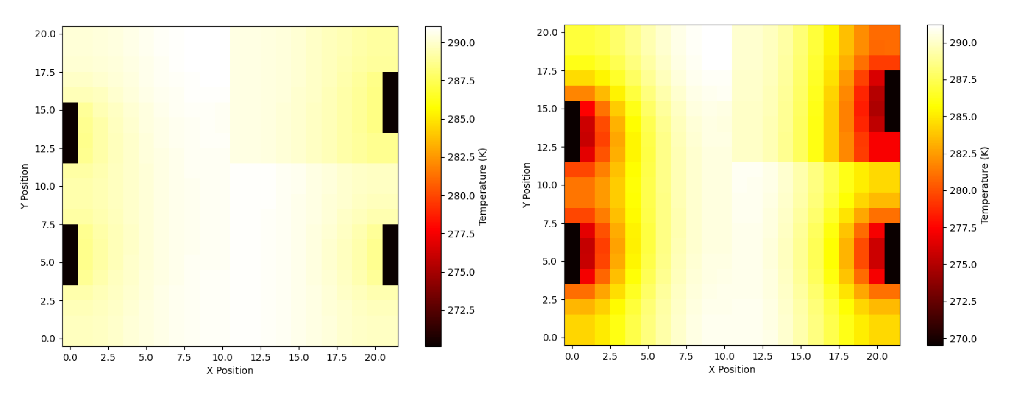
\includegraphics[width=\linewidth]{imgs_pres/wylaczanie_grzejnikow_temp_ostateczne.png}
        \label{fig:enter-label}
    \end{figure}
\end{frame}

\begin{frame}{Jak ogrzać zimne pokoje??}
    \begin{figure}[ht]
        \centering
        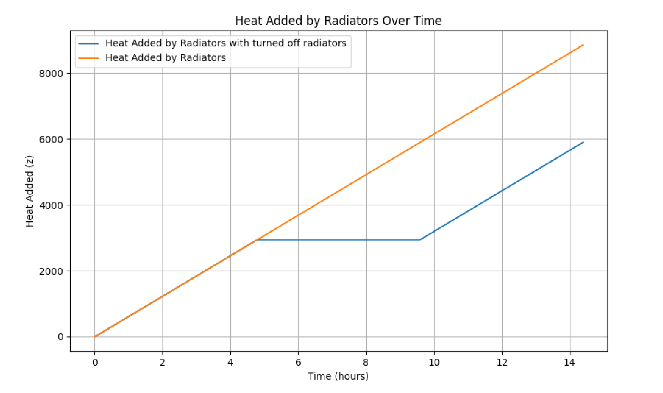
\includegraphics[width=\linewidth]{imgs_pres/wylaczanie_grzejnikow_energie.png}
        \label{fig:enter-label}
    \end{figure}
\end{frame}

\begin{frame}{The end}
    \centering Dziękuję za uwagę!!!
\end{frame}

\end{document}
